\documentclass[12pt]{article}
\usepackage[spanish]{babel}
\usepackage{listings}
\usepackage{array}
\usepackage{graphicx}

%opening
\title{{\Huge \textbf{Mips}}}
\author{Samuel Primera CI: 31.129.684}

\begin{document}
	\maketitle
	
	
	\section{Repertorio de Instrucciones}
	
	El repertorio de instrucciones de un procesador es el conjunto de operaciones que pueden ejecutarse directamente en el hardware. Estas instrucciones incluyen cálculos aritméticos, manipulaciones de memoria y control de flujo de ejecución.
	
	Los lenguajes de programación de alto nivel como \textbf{C o Java} permiten a los desarrolladores escribir código de manera más intuitiva. Sin embargo, para que el hardware ejecute estos programas, el código debe traducirse a lenguaje ensamblador y luego a lenguaje de máquina.
	\\
	
	El proceso de traducción ocurre en varias etapas:
	\begin{enumerate}
		\item \textbf{Código fuente}: Escrito en un lenguaje como C.
		\item \textbf{Lenguaje ensamblador}: Representa instrucciones en un formato más cercano al hardware.
		\item \textbf{Lenguaje de máquina}: Conjunto de bits interpretados por el procesador.
	\end{enumerate}
	
	\section{Operaciones en MIPS}
	
	MIPS es una arquitectura basada en el paradigma \textbf{RISC (Reduced Instruction Set Computing)}, lo que implica un repertorio de instrucciones simplificado, con una estructura clara y uniforme.
	\\\\\\
	Ejemplo de suma en lenguaje ensamblador:
	\begin{lstlisting}
	add a, b, c   # Suma b y c, almacena el resultado en a
	\end{lstlisting}
	En MIPS, cada instrucción:
	\begin{itemize}
		\item Ejecuta \textbf{una sola operación}.
		\item Tiene \textbf{exactamente tres operandos} (dos fuentes y un destino).
		\item Se estructura de manera predecible para optimizar el hardware.
	\end{itemize}
	
	Si se requiere la suma de cuatro variables, se emplean varias instrucciones:
	
	\begin{lstlisting}
	add a, b, c   # Suma b y c
	add a, a, d   # Suma el resultado anterior con d
	add a, a, e   # Suma el resultado anterior con e
	\end{lstlisting}
	
	Este diseño permite una implementación eficiente en hardware, simplificando los circuitos y mejorando la velocidad de ejecución.
	
	\subsection{Operandos Mips}
	
	\begin{flushleft}
	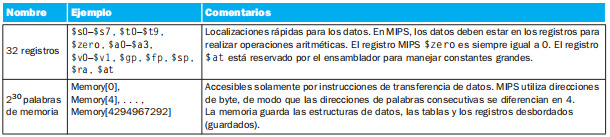
\includegraphics[width=1.2\linewidth]{OperandosMips.jpg}
	\end{flushleft}
	
	\subsection{Lenguaje Esamblador Mips}
	
	\begin{flushleft}
		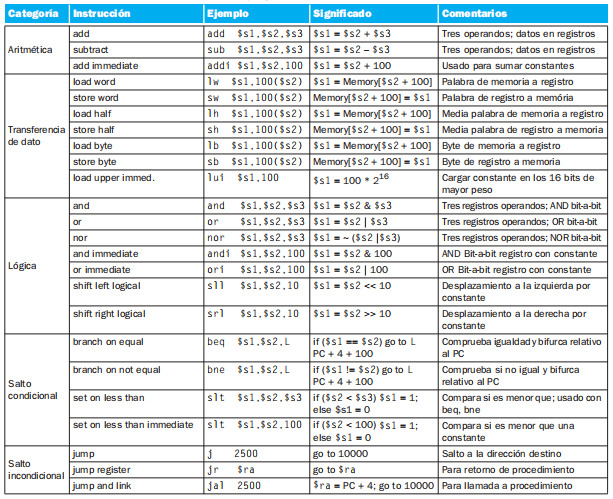
\includegraphics[width=1.2\linewidth]{LenguajeEsambladorMips.jpg}
	\end{flushleft}
	
	
\end{document}